\newpage
\section{Introduction}
\label{sec:introduction}

% state the learning objective 
\par In this laboratory assignment, a circuit containing both an independent (first constant and then sinusoidal) and a current controlled voltage sources ($V_s$ and $V_d$, respectively), a voltage controlled current source ($I_b$), connected to multiple resistors (from $R_{1}$ to $R_{7}$) and a capacitor ($C$) is going to be studied. The described circuit can be observed in detail in Figure~\ref{fig:rc}.

\par In Section~\ref{sec:theoretical}, a theoretical analysis of the circuit is presented, studying the static, time and frequency responses, using the Octave tool. After that, in Section~\ref{sec:simulation}, the circuit is analysed via simulation, using the software Ngspice. The obtained results are then compared, explaining the reasons behind the differences and similarities found. Finally, one can find the conclusions of this study outlined in Section~\ref{sec:conclusion}.

\begin{figure}[h] \centering
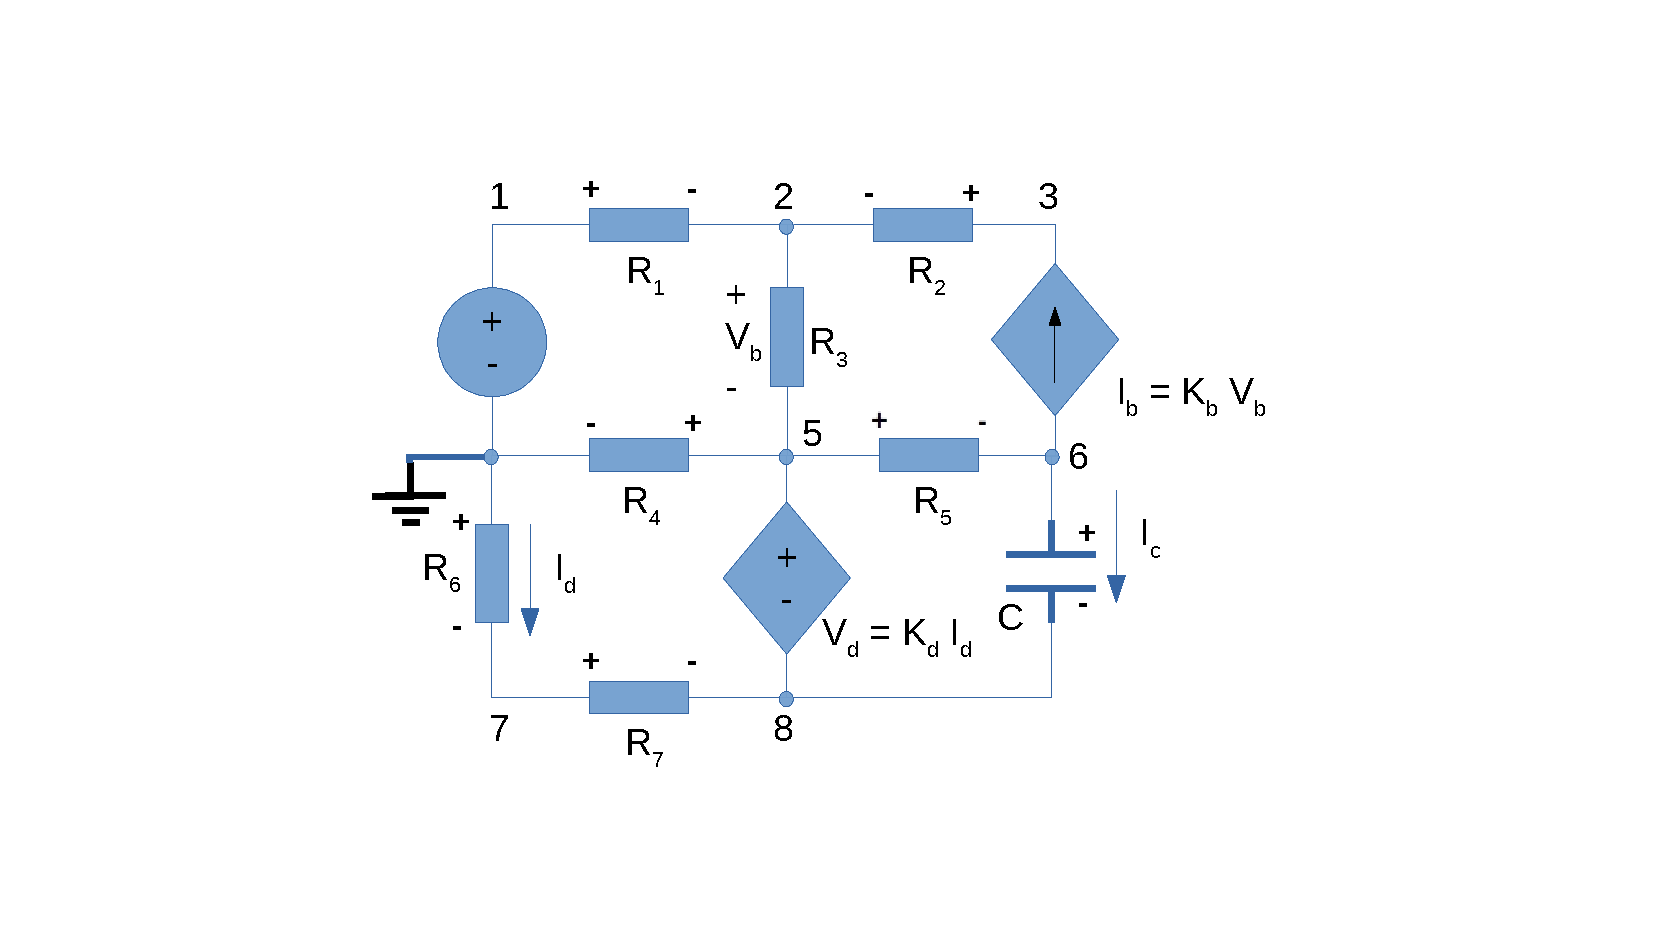
\includegraphics[width=1.1\linewidth]{rc.pdf}
\caption{Circuit diagram.}
\label{fig:rc}
\end{figure}
